\newcommand{\templatesdir}{../../../templates}
\newcommand{\template}{template-roteiro-est}
\input{\templatesdir/\template/template}

\newcommand{\content}{Filas de prioridade}
\newcommand{\class}{Algoritmos e Estruturas de Dados}
\newcommand{\shortcourse}{45EST}

\begin{document}

\makeheader

{
Leitura obrigatória:
\begin{itemize}
	\item Capítulo 9 de~\cite{GoodrichEtAl2014} -- Filas de prioridade.
\end{itemize}

Leitura complementar:
\begin{itemize}
	\item Capítulo 6 de~\cite{SzwarcfiterAndMarkenzon1994} -- Listas de prioridades.
	\item Capítulo 11 de~\cite{Preiss2001} -- Heaps e filas de prioridade.
\end{itemize}
}

\medskip

\newtitle{Filas de prioridade}

Ideia geral:
\begin{itemize}
	\item Cada elemento da fila tem um valor prioridade.
	\item A remoção é feita pela ordem de prioridade.
	\item Exemplos:
	\begin{itemize}
		\item Controle de tráfego aéreo.
		\item Fila de um banco com clientes preferenciais.
	\end{itemize}
\end{itemize}

\medskip

Funcionamento:
\begin{itemize}
	\item A fila armazena uma \textbf{entrada} com dois campos: chave e valor.
	\item Chave: prioridade do elemento.
	\item Valor: elemento armazenado.
	\item Elemento de menor chave possui prioridade.
	\item Métodos:
	\begin{itemize}
		\item \texttt{insert(k,\,v)}, \texttt{min()}, \texttt{removeMin()}.
	\end{itemize}
\end{itemize}

\medskip

\begin{figure}[H]
	\centering
	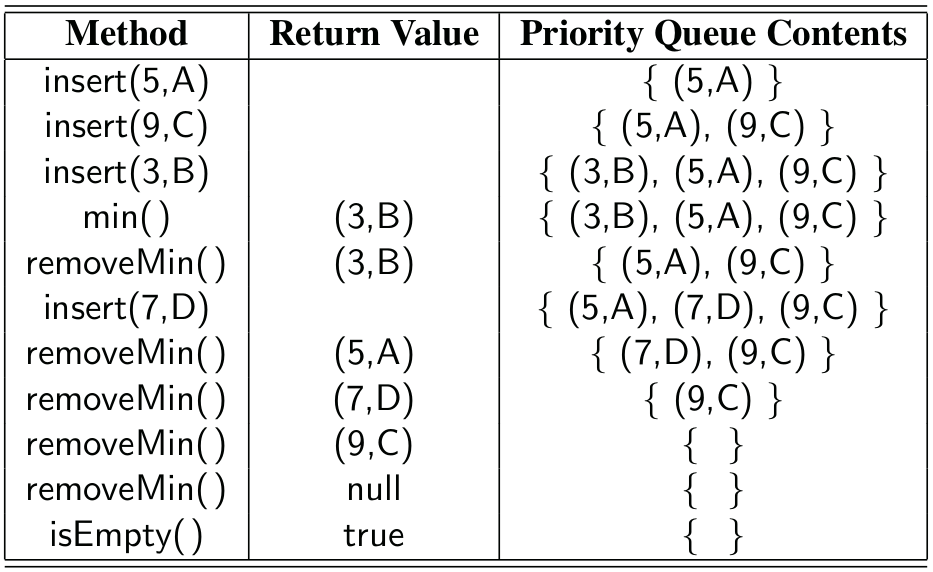
\includegraphics[width=0.6\linewidth]{img/table-9-1}
\end{figure}

{\color{redtext}
Detalhes:
\begin{itemize}
	\item Várias entradas com mesma chave $\to$ escolhe aleatoriamente.
	\item Chave não precisa ser numérica (ex: pode ser um tipo estruturado).
\end{itemize}
}

\medskip

Interface \texttt{Entry}:
\begin{minted}{java}
public interface Entry<K, V> {
	K getKey();
	V getValue();
}
\end{minted}

\medskip

Interface \texttt{PriorityQueue}:
\begin{minted}{java}
public interface PriorityQueue<K, V> {
	int size();
	boolean isEmpty();
	Entry<K,V> insert(K k, V v);
	Entry<K,V> min();
	Entry<K,V> removeMin();
}
\end{minted}

\medskip

{\color{redtext}
Comentários:
\begin{itemize}
	\item Uma fila de prioridades armazena uma coleção de entradas e fornece métodos de acesso a elas.
	\item Para isso, usa internamente alguma estrutura de dados básica.
\end{itemize}
}

\bigskip

Comparação de chaves:
\begin{itemize}
	{\color{redtext}\item As chaves precisam ser comparáveis, formando uma ordem de elementos.}
	\item Opção 1:
	\begin{enumerate}
		\item Definir a classe da chave como comparável (\texttt{Comparable}) e implementar o método \texttt{compareTo}.
		{\color{redtext}
		\begin{itemize}
			\item Muitas classes do Java já são comparáveis, como \texttt{Integer}.
		\end{itemize}
		}
		\item Utilizar uma classe \texttt{Comparator} genérica para qualquer chave comparável.
	\end{enumerate}
\end{itemize}

\medskip

Classe comparadora genérica (\texttt{DefaultComparator}):
\begin{minted}{java}
public class DefaultComparator<E> implements Comparator<E> {
	public int compare(E a, E b) {
		return ((Comparable<E>) a).compareTo(b);
	}
}
\end{minted}

\medskip

\begin{itemize}
	\item Opção 2:
	\begin{enumerate}
		\item Criar uma classe \texttt{Comparator} específica para a chave usada.
	\end{enumerate}
\end{itemize}

\clearpage

Exemplo de comparador para tamanho de String:
\begin{minted}{java}
public class StringLengthComparator implements Comparator<String> {
	public int compare(String a, String b) {
		if(a.length() < b.length())
			return -1;
		else if(a.length() == b.length())
			return 0;
		else
			return 1;
	}
}
\end{minted}

\medskip

{\color{redtext}
Comentários:
\begin{itemize}
	\item Ao comparar dois elementos $a$ e $b$:
	\begin{itemize}
		\item Retorno $-1$ se $a < b$.
		\item Retorno $1$ se $b < a$.
		\item Retorno $0$ se $b = a$.
	\end{itemize}
\end{itemize}
}

\medskip

Implementação de uma fila de prioridade \textit{não ordenada}:
\begin{minted}{java}
public class UnsortedPriorityQueue<K, V>
	implements PriorityQueue<K, V> {
	
	protected static class PQEntry<K,V> implements Entry<K,V> {
		private K k;
		private V v;
		
		public PQEntry(K key, V value) {
			k = key;
			v = value;
		}
		
		public K getKey() { return k; }
		public V getValue() { return v; }
		protected void setKey(K key) { k = key; }
		protected void setValue(V value) { v = value; }
	}
	
	private PositionalList<Entry<K,V>> list = 
		new LinkedPositionalList<>();
	private Comparator<K> comp;
	
	public UnsortedPriorityQueue() {
		this(new DefaultComparator<K>());
	}
	
	public UnsortedPriorityQueue(Comparator<K> c) {
		comp = c;
	}
	
	protected int compare(Entry<K,V> a, Entry<K,V> b) {
		return comp.compare(a.getKey(), b.getKey());
	}
	
	protected boolean checkKey(K k) {
		try {
			return (comp.compare(k, k)) == 0;
		} catch(ClassCastException e) {
			throw new IllegalArgumentException("Incompatible key");
		}
	}
	
	public boolean isEmpty() {
		return size() == 0;
	}
	
	private Position<Entry<K, V>> findMin() {
		Position<Entry<K,V>> small = list.first();
		Position<Entry<K,V>> walk = small;
		while(walk != null) {
			if(compare(walk.getElement(), small.getElement()) < 0)
				small = walk;
			walk = list.after(walk);
		}
		return small;
	}
	
	public Entry<K, V> insert(K k, V v) {
			
		checkKey(key);
		Entry<K,V> newest = new PQEntry<>(key, value);
		list.addLast(newest);
		return newest;
	}
	
	public Entry<K, V> min() {
		if(list.isEmpty()) return null;
		return findMin().getElement();
	}
	
	public Entry<K, V> removeMin() {
		if(list.isEmpty()) return null;
		return list.remove(findMin());
	}
	
	public int size() { return list.size(); }
	
	public String toString() {
		StringBuilder sb = new StringBuilder("(");
		Position<Entry<K,V>> walk = list.first();
		while(walk != null) {
			sb.append(walk.getElement().getValue() + " [" + walk.getElement().getKey() + "]");
			walk = list.after(walk);
			if (walk != null)
			sb.append(", ");
		}
		sb.append(")");
		return sb.toString();		
	}
}
\end{minted}

\medskip

{\color{redtext}
Comentários:
\begin{itemize}
	\item A classe \texttt{PQEntry} modela entradas \texttt{<chave, valor>}.
	\item As entradas são armazenadas em uma lista posicional.
	\item A fila possui um comparador \texttt{comp}. Ele é recebido como argumento na construção da fila, ou é atribuído o construtor \textit{default} predefinido.
	\item O método \texttt{checkKey} verifica se a chave é comparável.
	\item O método \texttt{findMin} busca elemento mínimo, a ser retornado/removido nos métodos \texttt{min} e \texttt{removeMin}.
\end{itemize}
}

\medskip

Implementação de uma fila de prioridade \textit{ordenada}:
\begin{minted}{java}
public class SortedPriorityQueue<K,V> 
	implements PriorityQueue<K, V> {
	
	protected static class PQEntry<K,V> implements Entry<K,V> {
		private K k;
		private V v;
		
		public PQEntry(K key, V value) {
			k = key;
			v = value;
		}
		
		public K getKey() { return k; }
		public V getValue() { return v; }
		protected void setKey(K key) { k = key; }
		protected void setValue(V value) { v = value; }
	}
	
	private PositionalList<Entry<K,V>> list = 
		new LinkedPositionalList<>();
	private Comparator<K> comp;
	
	
	public SortedPriorityQueue() {
		this(new DefaultComparator<K>());
	}
	
	public SortedPriorityQueue(Comparator<K> c) {
		comp = c;
	}
	
	protected int compare(Entry<K,V> a, Entry<K,V> b) {
		return comp.compare(a.getKey(), b.getKey());
	}
	
	protected boolean checkKey(K k) {
		try {
			return (comp.compare(k, k)) == 0;
		} catch(ClassCastException e) {
			throw new IllegalArgumentException("Incompatible key");
		}
	}
	
	public boolean isEmpty() {
		return size() == 0;
	}
	
	public Entry<K,V> insert(K key, V value) {
		
		checkKey(key);
		Entry<K,V> newest = new PQEntry<>(key, value);
		Position<Entry<K,V>> walk = list.last();
		
		while (walk != null && compare(newest, walk.getElement()) < 0)
			walk = list.before(walk);
		if (walk == null)
			list.addFirst(newest);
		else
			list.addAfter(walk, newest);
		return newest;
	}
	
	public Entry<K,V> min() {
		if (list.isEmpty()) return null;
		return list.first().getElement();
	}
	
	public Entry<K,V> removeMin() {
		if (list.isEmpty()) return null;
		return list.remove(list.first());
	}
	
	public int size() { return list.size(); }
	
	public String toString() {
		StringBuilder sb = new StringBuilder("(");
		Position<Entry<K,V>> walk = list.first();
		while(walk != null) {
			sb.append(walk.getElement().getValue() + " [" + walk.getElement().getKey() + "]");
			walk = list.after(walk);
			if (walk != null)
			sb.append(", ");
		}
		sb.append(")");
		return sb.toString();		
	}
}
\end{minted}

\medskip

{\color{redtext}
	Comentários:
	\begin{itemize}
		\item Diferente da fila não ordenada, o método \texttt{insert} adiciona a entrada de forma ordenada, do menor ao maior valor de chave.
		\item O elemento mínimo é o armazenado na primeira posição da lista.
	\end{itemize}
}

\medskip

Comparação de performance:

\begin{table}[H]
	\centering
	\renewcommand{\arraystretch}{1.2}
	\begin{tabular}{lcc}
		\hline
		Método & \texttt{UnsortedPriorityQueue} & \texttt{SortedPriorityQueue} \\
		\hline
		\texttt{size} & $O(1)$ & $O(1)$ \\
		\texttt{isEmpty} & $O(1)$ & $O(1)$ \\
		\texttt{insert} & $O(1)$ & $O(n)$ \\
		\texttt{min} & $O(n)$ & $O(1)$ \\
		\texttt{removeMin} & $O(n)$ & $O(1)$ \\
		\hline
	\end{tabular}
\end{table}

\medskip

\newtitle{Atividades}

\begin{enumerate}
	\item Implemente uma fila de prioridade para armazenar os passageiros de uma companhia aérea. Clientes do plano \textit{premium} possuem prioridade sobre clientes do plano \textit{basic}. Além disso, clientes \textit{prioritários} (idosos, gestantes, etc.) possuem ainda mais prioridade que clientes \textit{premium}. Crie um sistema para chamar os clientes para embarque pelo seu nome considerando a prioridade de cada um. Como critério de desempate dentro de um mesmo tipo, considere a idade do cliente.	Para modelar a prioridade (chave) utilize uma classe. Implemente usando filas ordenadas e não ordenadas.
	
	\bigskip
	
	\item Resolva os seguintes exercícios de~\cite{GoodrichEtAl2014}:
	\begin{itemize}
		\item[R-9.3:] O que cada uma das chamadas \texttt{removeMin} retorna, dentre a seguinte sequências de operações em uma fila de prioridade: \texttt{insert(5,\,A)}, \texttt{insert(4,\,B)}, \texttt{insert(7,\,F)}, \texttt{insert(1,\,D)}, \texttt{removeMin()}, \texttt{insert(3,\,J)}, \texttt{insert(6,\,L)}, \texttt{removeMin()}, \texttt{removeMin()}, \texttt{insert(8,\,G)}, \texttt{removeMin()}, \texttt{insert(2,\,H)}, \texttt{removeMin()}, \texttt{removeMin()}.
		
		\item[R-9.4:] Um aeroporto está desenvolvendo uma simulação computacional de controle de tráfego aéreo para lidar com eventos como aterrissagens e decolagens. Cada evento tem um \textit{timestamp} que simboliza o tempo em que o evento ocorrerá. A simulação necessita realizar eficientemente duas operações fundamentais:
		\begin{itemize}
			\item Inserir um evento com um \textit{timestamp} (isto é, adicionar um evento futuro).
			\item Retornar o evento com o \textit{timestamp} mais próximo (isto é, determinar o próximo evento para processar).
			\item Qual estrutura de dados deverá ser usada para realizar essas operações? Por quê?
		\end{itemize}
		
		\item[R-9.5:] O método \texttt{min} da classe \texttt{UnsortedPriorityQueue} executa em tempo $O(n)$. Faça uma pequena modificação na classe para que o método \texttt{min} execute em tempo $O(1)$. Explique qualquer modificação necessária em outros métodos da classe.
		
		\item[R-9.6:] Você pode adaptar sua solução do exercício anterior para fazer o método \texttt{removeMin} da classe \texttt{UnsortedPriorityQueue} executar em tempo $O(1)$? Justifique sua resposta.
		
		\item[R-9.12:] Considere uma situação onde um usuário possui chaves numéricas e deseja ter uma fila de prioridade \textit{orientada para o máximo}. Como pode uma fila de prioridade padrão (orientada ao mínimo) ser usada para tal propósito?
		
		\item[C-9.25:] Mostre como implementar uma pilha usando apenas uma fila de prioridade e uma variável inteira adicional.
		
		\item[C-9.26:] Mostre como implementar uma fila FIFO usando apenas uma fila de prioridade e uma variável inteira adicional.
		
		\item[C-9.27:] O Professor Idle sugere a seguinte solução para o exercício anterior. Sempre que uma entrada é inserida na fila, é dada uma chave que é igual ao tamanho atual da fila. Esta estratégia resulta em uma semântica FIFO? Prove que é verdadeiro ou dê um contra exemplo.
		
		\item[C-9.28:] Reimplemente a classe \texttt{SortedPriorityQueue} usando um array. Certifique-se de manter o desempenho do \texttt{removeMin} em $O(1)$.
	\end{itemize}
\end{enumerate}

\bigskip

\newtitle{Referências}
\begingroup
	\footnotesize
	\renewcommand{\chapter}[2]{}%
	\bibliographystyle{apalike}
	\bibliography{../referencias}
\endgroup

\end{document}